\documentclass[]{report}
\renewcommand\thesection{\arabic{section}}%for page numbering in arabics
\usepackage{graphicx,tabularx}%for figures and tables
\usepackage[utf8]{inputenc} %allows special characters such as ä, ö, ỳ
\usepackage[english]{babel}  %set the language to English
\usepackage[margin=1.5in]{geometry} %change page margins 
\usepackage{sectsty}%section headers
\allsectionsfont{\sffamily\huge}
\subsectionfont{\sffamily\LARGE}
\subsubsectionfont{\sffamily\large}
\linespread{1.2}% line distance
\usepackage{lipsum}% http://ctan.org/pkg/lipsum
\usepackage{caption}%use for captions on tables
%use this exact command. The style and bibliographystyle has to be authoryear (Havard). The sorting is nyt: name, year, title so that the bibliography is sorted alphabetically. firstinits=true shortens the names: Albert Einstein -> A. Einstein
\usepackage[backend=bibtex,style=authoryear,bibstyle=authoryear,sorting=nyt,firstinits=true]{biblatex}
\setlength\parindent{0pt}%include this so that your paragraphs don't indent automatically
\addbibresource{report.bib} %this attaches your bib-file, your bibliography (must be in the same folder)
\usepackage[compact]{titlesec}%include title formatting package
\usepackage{float}
\graphicspath{ {./images/} }

\setcounter{secnumdepth}{3}
\setcounter{tocdepth}{3}

% Title Page
\title{Git CLI or GitHub Desktop \\ What are the factors that influence the choice of the interface among IT students?}
\author{Danil Burov and Giulio Raffaeli}
\date{December 18th 2023\\Module: ARDA \\Venlo, Limburg, Netherlands}


\begin{document}
	
	\maketitle
	
	\begin{abstract}
		%history%
		When it comes to learning programming one of the main aspects an IT student needs to learn is how to version control (VS) their work. The most common tool for versioning is Git. In the beginning IT students need to choose between Command Line Interface (CLI) and Graphical User Interface (GUI) for Git usage. \\\\
		%cite -> wikipedia% 
		%topic introdutction%
		
		This purpose of this research is to identify what are the main factors that influences the choice of the interface among IT students. In order to evaluate the reasons, a survey was conducted. Since the most efficient way of using Git is through the CLI an experiment was done to understand why students adhere to the GUI instead switching to the more efficient interface.\\\\
		%data evaluation%
		The results show that the majority of IT students prefer using Git through the GUI, finding it more visual appealing and easier to understand. Even thought, students that CLI is more efficient using Git they still use the GUI because making the transition is harder than sticking to the interface. This statement is proven with our experiment.\\\\
		\pagenumbering{roman}
		
	\end{abstract}
	\tableofcontents
	\setcounter{page}{3}
	\listoffigures %UNCOMMENT IF YOU HAVE FIGURES
	%\listoftables %UNCOMMENT IF YOU HAVE TABLES
	\pagebreak
	
	\pagenumbering{arabic}	
	
	\section{Introduction}
	The purpose of this chapter is to provide the research question and the importance of it, along with context about the topic. Furthermore, this chapter will point out potential external factors that may influence the evaluation of the hypothesis and its sub-questions. \\
	\subsection{Context and Background}
	
	%Talk about how Git works%
	\subsubsection{Git}
	Up until this date Git is the most popular versioning control system, used by more than 93 percent of developers ('cite' -> StackOverflow survey). In order to understand Git it is crucial to know what is a versioning control system is (VCS). It is a system that enables developers to keep historical version of source code(*) and project files that are under development and retrieve past version. It is required when developing projects above a few hundred lines of code or where more than one developer needs to collaborate on a project. It stores version information for every file in what is generically called - 'repository'('cite -> pdf history of version control') . The basic structure of a Git repository has three main components. First, a .git directory which has the functionality of storing the meta data and object database for you repository and all the committed changes. Second, a staging area where new features that still need to be committed are kept, waiting for a commit to take place. Lastly, a working directory where your plain running copy of the source code is held. Once a commit takes place, the changes are saved from the staging area to the .git directory. ('cite -> pdf for CLI compare to GUI').
	
	\subsubsection{Command line Interface and Graphical User Interface}
	%Story CLI vs GUI%
	When the first personal computer was invented in 1973 (Kenbak - 1) ('cite' - > Museum computerhistory.org) users were forced to use the command line interface as their only way of interacting with the machine. Later on, with more people using the personal computers the need for a graphical user interface increased. The first prototypes of personal computers that use the GUI were developed in the 1970s (XEROX Alto 1973) ('cite' -> wikipedia), however, it became popular with the release of the 'Macintosh' in 1984. ('cite' ->wikipedia ). From that point on, the majority of users started using the GUI as their main interface relegating the use of CLI only to a small percentage of users.\\
	When Git was first released in 2005 ('cite' -> Gitpage) the only way to work with it was through the command line interface. Throughout the years many graphical user interfaces supporting Git were developed with the most important one being GitHub Desktop, created in 2017. ('cite' -> GitHub page)
	
	%How they work with Git%
	%Which one is more efficient%
	%two of the main limiting factors when it comes to the GUI
	When using the command line interface you type commands manually to perform the desired actions whilst in a graphical user interface you will have something visual to interact with, such as buttons, input fields and so on. There are advantages and disadvantages of using either of the two interfaces not only for Git but in general. ('cite' -> pdf for CLI vs GUI). When it comes to programming, 83('cite' -> StackOverflow survey) percent of developers prefer the CLI instead of the GUI for various of reasons. Here are some of them: \\1) Interaction speed, when it comes to GUI the speed is determined mostly on how fast you can navigate with your mouse and click speed while with the CLI what you need to do is just interact with the keypad making the process faster. \\2) Efficiency, because of the way interaction is handled in the GUI it also requires more actions compared to the CLI to execute the same task. For example: If you want to commit changes to the main repository with the CLI you need to execute three consecutive commands, whereas in the GUI you need to navigate through three different buttons and you have to input a message with your keyboard. \\3) One complaint about CLI tools is that they supposedly have a 'steeper learning curve' and no one can remember what commands to use. However, if you need to learn a complex GUI the 'learning curve' can be as steep as learning the CLI. Although, in the long run it is always better to the learn the CLI because more efficient. ('cite' -> github repo)

	%Reasearch question% 
	%hypothesis -> X -> Y potential C's and I's%
	\subsection{Research questions and Hypothesis}
	The aim of the research is to find what are the reasons that influence the choice of the interface among IT students. Therefore our research questions is: "What are the factors that influence the choice of the interface among IT students?". Since surveys show that command line interface is more used ('cite' -> StackOverflow ) than graphical user interface ('cite' -> GitHub repo) and also more efficient the sub-question this research paper is aiming to answer is the following: "Is transitioning to the CLI hard for an IT student that still uses the GUI?".
	
	We hypothesis that students do not base their choice of Git interface on efficiency but on how user-friendly and simple the interface is. Therefore, we also believe that making the transition to the CLI from GUI is hard, because of the steep learning curve from the beginning and that is why IT students keep using the GUI.\\
	Although, there are some external factors that need to be taken into consideration. \\1) The years a student has already programmed for.\\2) How long have they been working with Git. \\3) What was their first chosen interface.\\4) Which operating system do they use. 
	
	In order to take into consideration the given factors a survey was conducted to evaluate what are the aspects that influence the choice of interface for an IT student. Parallel to the survey, an experiment was conducted with students that have never used the CLI before in order to understand what difficulties they will encounter when learning basic commands and if it makes them faster at using Git. 
	
	%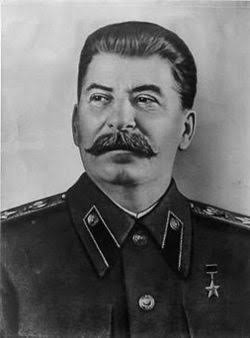
\includegraphics{test}
	\section{Methodology}
	This chapter will explain how we performed our research and how we set up our comparative analysis.
	
	\subsection{Gathering data}
	Since our research aims to find  on what do IT students base their choice of interface we had to gather all the data mainly by ourselves and some external sources.  This data has been gathered through the survey and experiment that was conducted among them.
	\subsubsection{Survey}
	
	In order to answer our main question, while also keeping in consideration all the external variables that may influence the answer, a survey was conducted.
	Since the research aims to give an answer that represents all IT students, the survey was sent not only to Fontys learners, but also to students from other universities.
	The survey itself consists of 14 multiple choice questions, plus an optional open question. It is structured as follows:\\
	First of all general questions are asked, regarding how long has the participant programmed for, how long has he been using Git and what is his current knowledge of the tool.
	Next questions are related to which Operating System does the responder primarily use and how did he get into Git at first (from which sources did he learn to use it and with which interface).
	Afterwards, information regarding which interface does the participant currently use and why is gathered
	Subsequently, the respondent needs to associate various words to both interfaces, in order to understand what is his opinion on them.
	Lastly, questions about whether the candidate has ever considered switching interface and if he thinks that doing so would improve his efficiency are asked.
	In order to easily convert all the answers into data, the survey was created with the tool Google Forms (Google - 2008).
	The list of all the questions and the possible replies can be found in the appendix.
	
	\subsubsection{Experiment}
	
	%i have stated that experienced users have conducted the experiment as well and results show that since they have prior knowledge with the CLI it was easier for them to complete the exercise without any problem%
	
	%i will specify that we have made an experiment with 5 people that have never used Git with CLI and 5 people who have already used Git with CLI%
	The experiment was conducted among second year IT students from Fontys. Given this information we chose the GUI to be GitHub Desktop since it is the most used graphical user interface.
	%the purpose of the assignment%
	
	
	The main purpose for the experiment conducted for our research paper is to prove that when a person wants to switch from using the graphical user interface (GitHub Desktop) for Git to the command line interface the transition will take time and effort when it comes down to getting used to the commands. Especially because as mentioned above the learning curve is very steep. ('cite' -> GitHub repo).
	
	%explaining why we are doing two experiments with gui and cli and why we are doing the assignment briefly%
	The exercise given to the students represent a very simple scenario where a developer would need to use Git through their interface. For the sake of our paper the experiment was done through both the graphical user interface and the command line. For a GUI we chose to use 'GitHub Desktop' since it is the most commonly used graphical interface ('cite' -> find somewhere to cite from this quote). The purpose of doing the assignment in both the interfaces is to prove that using the CLI for Git is much slower for students who have never used it and much more confusing. However, when a student had already used the CLI for Git purposes it was seen that the issues the newcomers had (mainly commands) weren't in the picture.\\
	
	%explaining the assignment%
	The assignment is covering all the basic commands that need to be done in order to complete a commit changes in a repository. Both groups of IT students have never seen the assignment and were treated as they have never used Git through the CLI. They were given two sheets of paper and a repository containing the assignment they need to complete. The first paper, contained all the commands required to complete the assignment ('refer to a figure').The second paper, had the description of the assignment.('refer to a figure here'). Time was recorder during the conducting of the exercises.
	
	
	\subsection{Data visualization and transformation}
	After gathering all the data, in order to store it in an organized way, multiple sheets were created. The tool used to create them was 'Google Sheets'. After inserting the data gathered from the survey it was exported as a 'CSV' file in order to use it later on for the data transformation. The same process was executed for the experiment. \\
	
	To perform the data transformation we had to choose between 'Python' and 'R'. We chose to use 'Python' with the library "pandas" v2.1.4 (McKinney, 2023) because we had previous knowledge of the language. \\
	
	First of all, we had to convert our 'CSV' files into dataframes which can then be used to generate plots with the use of the library "plotnine" v0.10.4 (Kibirige, 2023).  With this library multiple type of charts were created based on the variables that needed to be visualized or compared. One of the created diagram is the histogram. It was used to visualize single variable plots. The second type of diagram is the bar chart. We used it to display comparison between different entries of the same variable. And lastly, bar charts with multiple variables were used to point out correlations within two parameters.
	
	Before creating the plots, we needed to refine our dataframe. Initially, we had to remove a column named 'Timestamp' which was generated automatically while converting the survey data from 'Google Forms'. Later on, to perform specific queries we had to filter the data based on particular factors which influenced greatly the outcome of our plots. Moreover, to count how many times each word was chosen we needed to separate group of words and evaluate each one individually. Lastly, for the experiment dataframe we had to calculate the average time of completion for both interfaces to have a clear view of the time difference
	\section{Results}
	In this section we are going to display and explain each diagram that was generated from the results of the survey and the experiment. Every diagram will have a short explanation why it was created and the impact it has for our research. The survey had 60 participants while the experiment had 10 candidates. 
	
	\subsection{Survey participant information}
	%FINISHED
	In this subsections plots containing general programming expertise of the participants are going to be displayed, as well as their git experience and the interface they commonly use.\\
	
	As we can see from the figure below, among all the participants the majority of them (25) has been programming for 1-2 years, followed by 5+ years experience (24). Only, a small group of students has been programming for 2-5 years (9). (Figure.1)
	
	\begin{figure}[H]
		\centering
		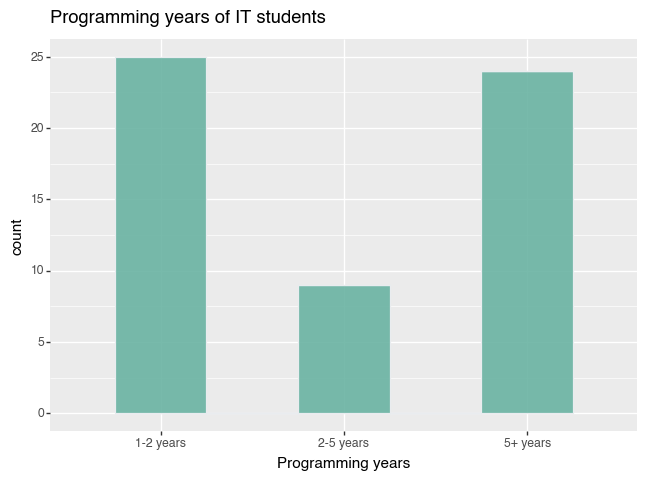
\includegraphics[width=0.75\linewidth]{ProgrammingYears}\\
		\caption{Programming years}
		\label{fig:  1}
	\end{figure}
	
		The diagram shows that 31 participants have been using Git for 1-2 years. 19 participants between 3-5 years and only 9 students have answered more than 5 years. (Figure. 2)
	\begin{figure}[H]
		\centering
		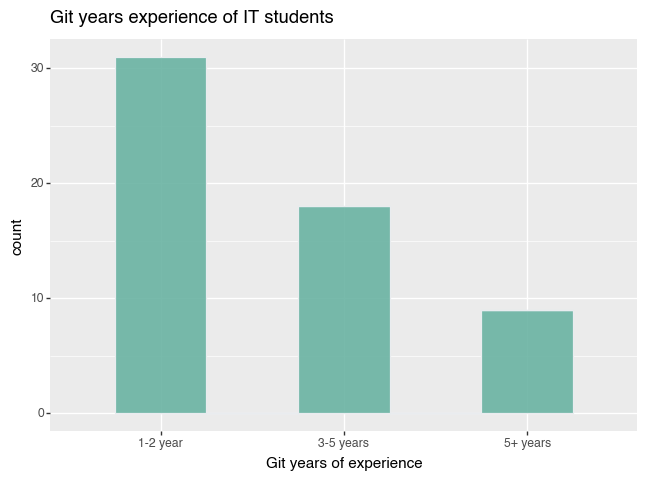
\includegraphics[width=0.75\linewidth]{GitYearsExperience}
		\caption{Git years of experience}
		\label{fig: 2}
	\end{figure}
	
	In the figure below, the results of which is the most preferred interface is shown. From the diagram (Figure. 3) it is very clear that most of the participants of our survey use the graphical user interface instead of the command line.
	
	
	\begin{figure}[H]
		\centering
		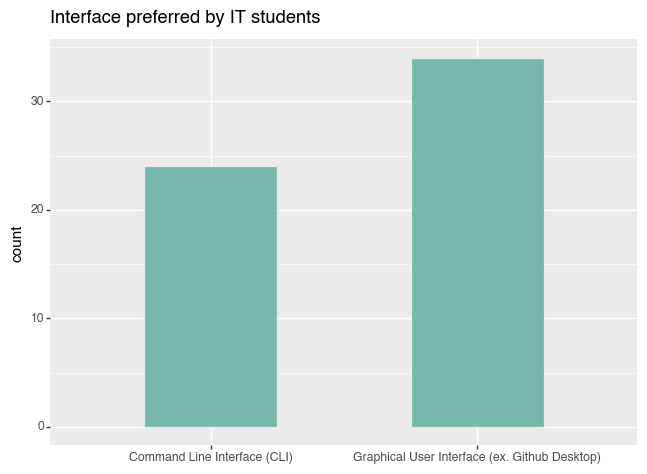
\includegraphics[width=0.75\linewidth]{preferredInterface}
		\caption{Preferred interface}
		\label{fig: 3}
	\end{figure}
	
	%END
	
	%Danny
	\subsection{Reasons to choose each interface}
	The plots displayed in this subsection will display the factors that influenced the student to choose the interface they are currently using. They had to select from a range of words that represent why they opted for the interface they are currently using. We have two plots which show the answers from graphical user interface users and command line interface users. \\
	
	The following figure (figure.4) , presents the response of the IT students using the GUI as their main interface for usage with Git. It specifically highlights the words they associate with the GUI.
		\begin{figure}[H]
		\centering
		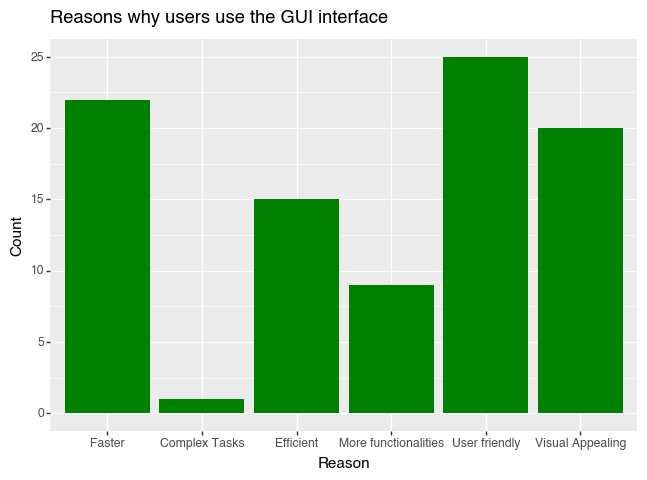
\includegraphics[width=0.75\linewidth]{ReasonsGUI}
		\caption{Reasons why students choose GUI}
		\label{fig: 4}
	\end{figure}
	
	The figure below (figure.5) showcases the feedback from IT students who predominantly use the command line interface (CLI) for Git operations. It focuses mainly on the words the students used to associate their Git usage via the CLI. 
	
	\begin{figure}[H]
		\centering
		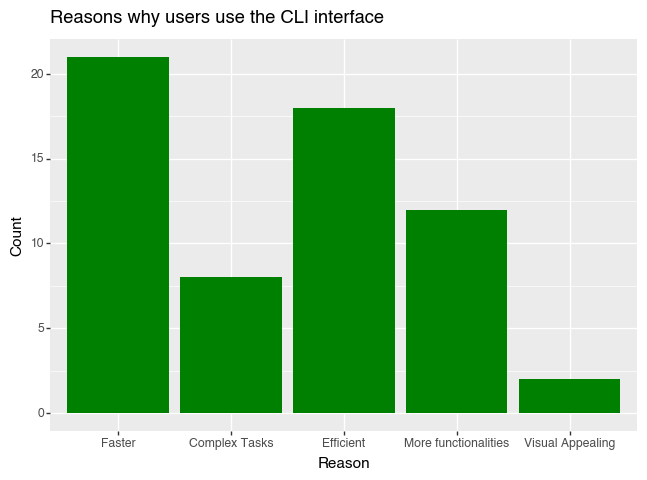
\includegraphics[width=0.75\linewidth]{ReasonsCLI}
		\caption{Reasons why students choose CLI}
		\label{fig: 5}
	\end{figure}
	
	%Danny
	\subsection{External factors that influence the choosing }
	Here we have derived all the external factors that influences the choice of the IT student's interface.  We evaluated if the time spent in Git, the operational system that the student uses and years of Git experience, influence the interface of their choosing.\\
	
	In Figure.6 it is shown that the majority of the IT students who did the survey use the operational system 'Windows'. Whereas the 'Mac' and 'Linux' OS is not that common among the students. Most of the people who use 'Windows' use the graphical user interface to operate with Git. And we can see that the other two operational system have very similar results when it comes down to choosing their interface for Git usage.
	
		\begin{figure}[H]
			\centering
			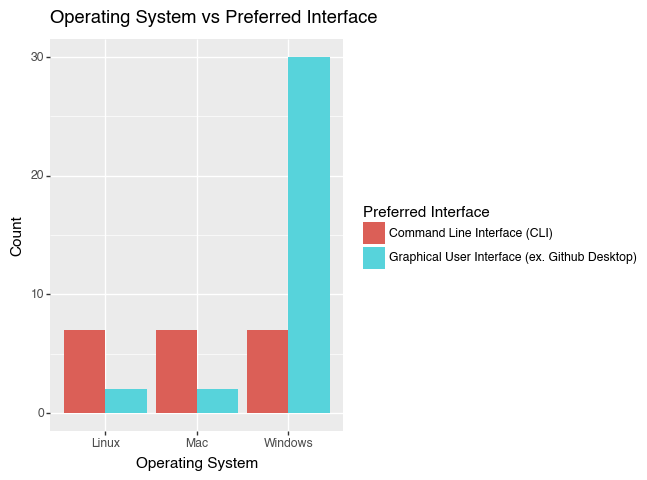
\includegraphics[width=0.75\linewidth]{OSAffectsInterface}\\
			\caption{Operational system affecting the chosen interface}
			\label{fig: 6}
		\end{figure}
		
		The time that a student spends in Git is crucial in choosing the interface. In figure.7 we have displayed the times that IT students spent in Git, executing commands or in general working with Git in one hour.
			\begin{figure}[H]
			\centering
			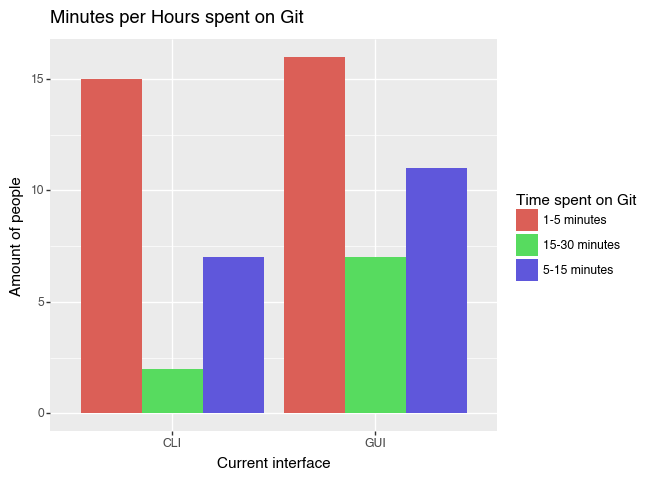
\includegraphics[width=0.75\linewidth]{TimeSpentGit}\\
			\caption{How much time do the students spent on Git}
			\label{fig: 7}
		\end{figure}
		
		The following factor is answering if whether the years a student has been using Git has any sort of impact of their choosing of the interface they are currently using.
		\begin{figure}[H]
			\centering
			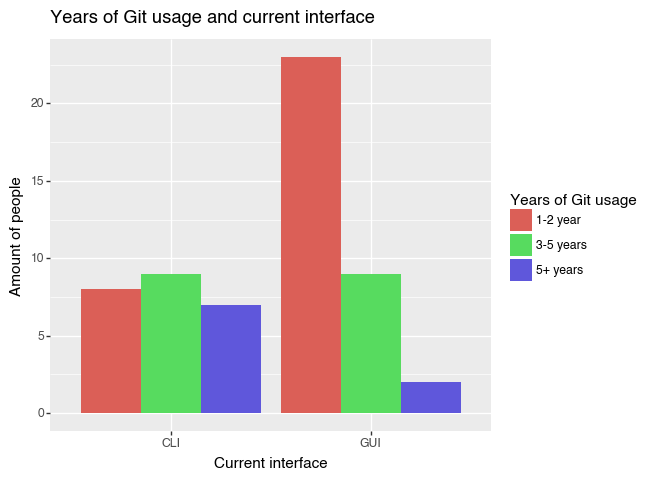
\includegraphics[width=0.75\linewidth]{YearsGitImpact}\\
			\caption{Impact of Git years on the interface}
			\label{fig: 8}
		\end{figure}
		
		%Giulio
		\subsection{Efficient usage of Git based on the interface}
		
		This section is going to display the  results about the reasons why a user would like to switch its interface. First of all, we are going to analyze, based on the current interface they use, whether they ever consider swapping to the other interface at one point of their programming career.
		Then, based on the question above, we are going to see if the participants believe that switching would improve their speed and efficiency, or if they stick to the current one because swapping would slow their process.\\\\
		
		From the first plot (Figure 9) we notice that the majority of CLI users (14 candidates) never thought of switching, while 10 of them wanted to use the other interface at least once
		
		\begin{figure}[H]
			\centering
			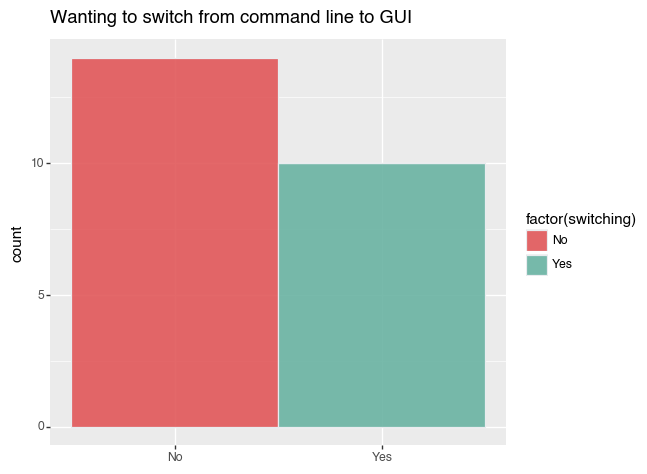
\includegraphics[width=0.75\linewidth]{SwitchingCLI}\\
			\caption{How many people want or have swapped from CLI to GUI}
			\label{fig:13}
		\end{figure}
		
		On the GUI side, 20 people stated that they never thought of swapping to CLI, while 14 candidates at least had this idea once.
		From both images (Figure 9 and Figure 10), we can see that the ratio is almost similar regardless of the interface
		
		\begin{figure}[H]
			\centering
			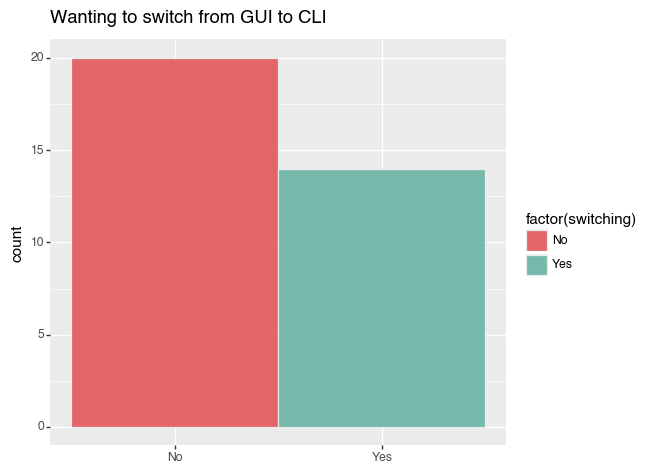
\includegraphics[width=0.75\linewidth]{SwitchingGUI}
			\caption{How many people want or have swapperd from GUI to CLI}
			\label{fig: 14}
		\end{figure}
		The following diagram (Figure 11) is used to display whether people that considered swapping believe that it will make them faster. From the result, all the candidates that answered (24), are convinced that swapping would not improve their speed at alll.
		\begin{figure}[H]
			\centering
			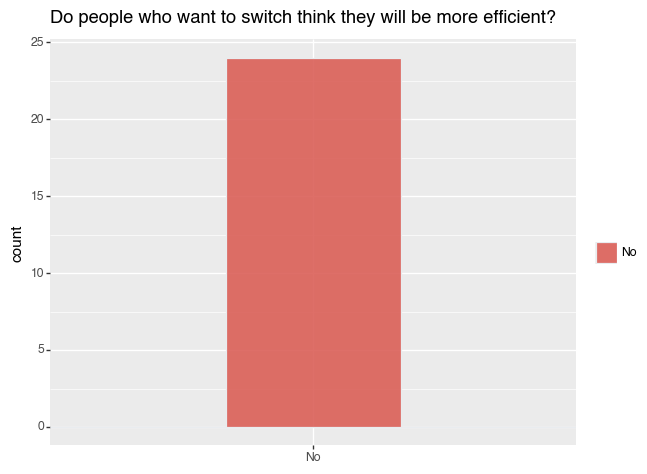
\includegraphics[width=0.75\linewidth]{EfficientSwitch}\\
			\caption{People who have switched (Efficiency)}
			\label{fig: 9}
		\end{figure}
		Confirming this opinion, people that never considered switching believe that they are using the faster method, while a small percentage (6 candidates) are doubtful about this statement
		\begin{figure}[H]
			\centering
			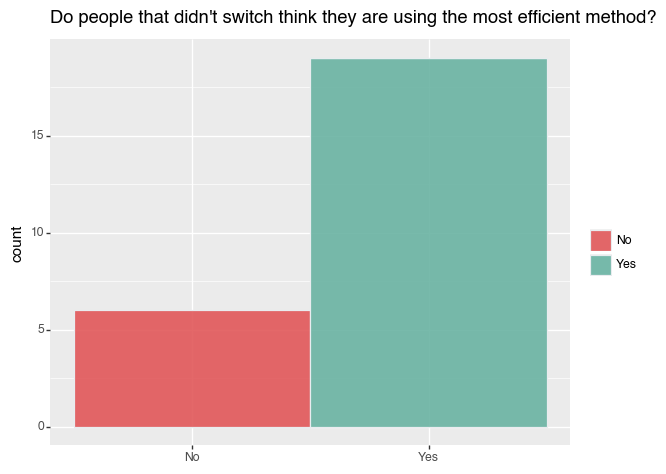
\includegraphics[width=0.75\linewidth]{EfficientNoSwitch}\\
			\caption{People who haven't switched (Efficiency)}
			\label{fig: 10}
		\end{figure}
		Following this trend, when people that want to switch are asked whether they will be faster with their new interface,  only 3 candidates believe that this is going to be the case, leaving the 21 remaining sceptical, as we can see from the diagrams below (Figure 13, Figure 14)
		\begin{figure}[H]
			\centering
			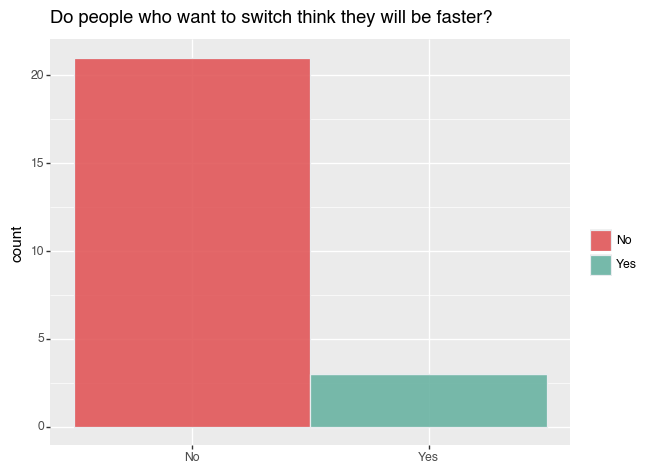
\includegraphics[width=0.75\linewidth]{SpeedSwitch}\\
			\caption{If people think that their interface is the fastest (Switch)}
			\label{fig:11}
		\end{figure}
		\begin{figure}[H]
			\centering
			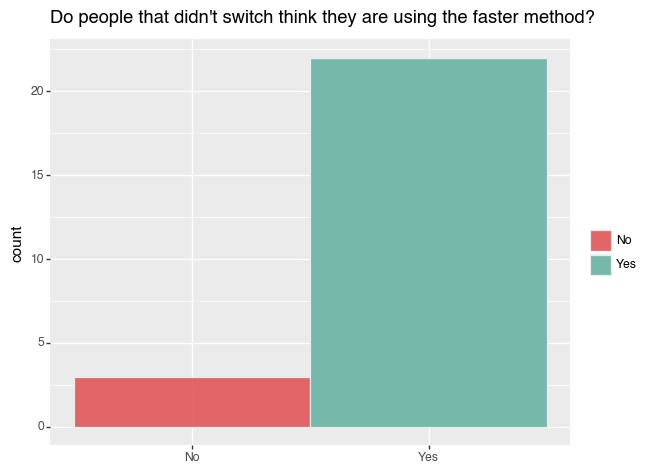
\includegraphics[width=0.75\linewidth]{SpeedNoSwitch}\\
			\caption{If people think that their interface is the fastest (No switch)}
			\label{fig: 12}
		\end{figure}
		
		
	
	%Giulio
	\subsection{Words association for the two interfaces}
	
	In this sections we are going to have a deep look at what are the most common words associated with both interfaces. In order to have a bigger picture in the end, we created 4 separated diagrams, the first one displaying what do people that use CLI think about their interface, followed by their opinion on GUI. Next, the results about which are the most common words associated to GUI from its audience and their thought about CLI are going to be presented.\\\\

	From the diagram below (Figure 15) we can acknowledge that 23 CLI users believe that the Command Line is more controlled, 21 that is more efficient and 15 that it helps to control and manage files better. Some of them also think that it is easy to use and helpful, but at the same time dispersive.
	\begin{figure}[H]
		\centering
		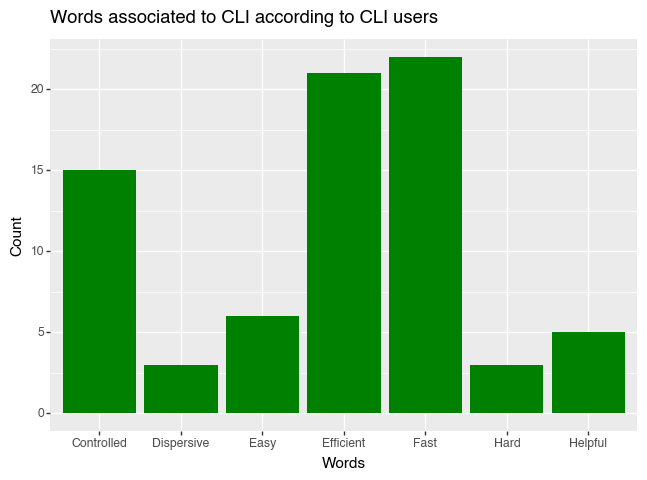
\includegraphics[width=0.75\linewidth]{WordsCLIFromCLI}\\
		\caption{What does a CLI user associate the CLI with}
		\label{fig: 15}
	\end{figure}
	
	On the other hand, from the following image(Figure 16) it is clear that the majority of CLI users ( 14 candidates) state that using the GUI is easier and helpful, but at the same time slower and more time consuming. Just a few participants believe that using the GUI is efficient, fast and controlled, while others said that is dispersive and hard.
	\begin{figure}[H]
		\centering
		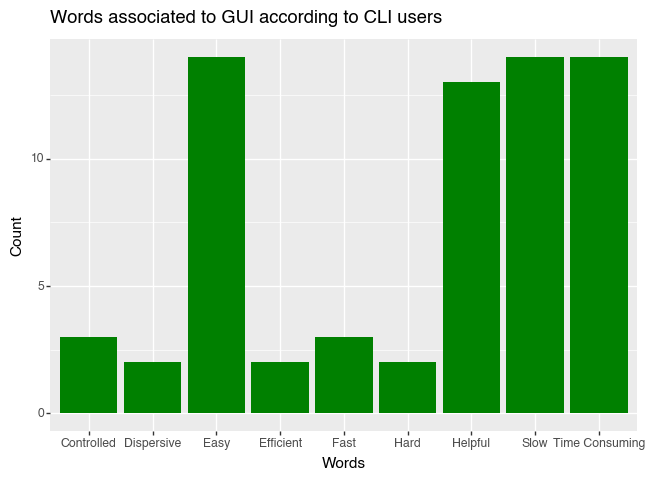
\includegraphics[width=0.75\linewidth]{WordsGUIfromCLI}\\
		\caption{GUI user words for CLI}
		\label{fig: 17}
	\end{figure}
	
	In the next diagram (Figure 17) we can see that the majority of GUI user's opinion(25 users) on their interface is that it's easy to use and helpful. Another big portion (15 people) believe that it is fast, efficient and controlled, although some of them also think that its is hard, slow, time consuming and dispersive
	
	\begin{figure}[H]
		\centering
		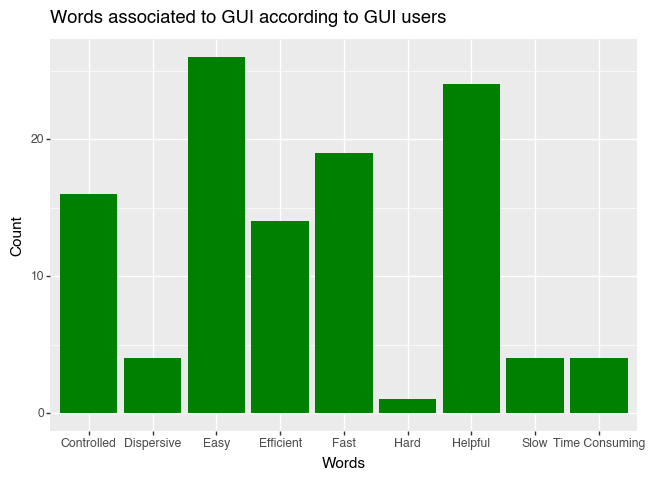
\includegraphics[width=0.75\linewidth]{WordsGUIfromGUI}\\
		\caption{What does a GUI user associate GUI with}
		\label{fig: 16}
	\end{figure}
	
	In the last image (Figure 18), we can notice that a lot of GUI users (31 candidates), still acknowledge the fact that CLI is more efficient, fast and controlled(14 users). However, they also state that it is hard, time consuming (16 participants) and dispersive. Lastly, a smoll portion (4 people) claims that this interface is easy and helpful to use.
	
	
	\begin{figure}[H]
		\centering
		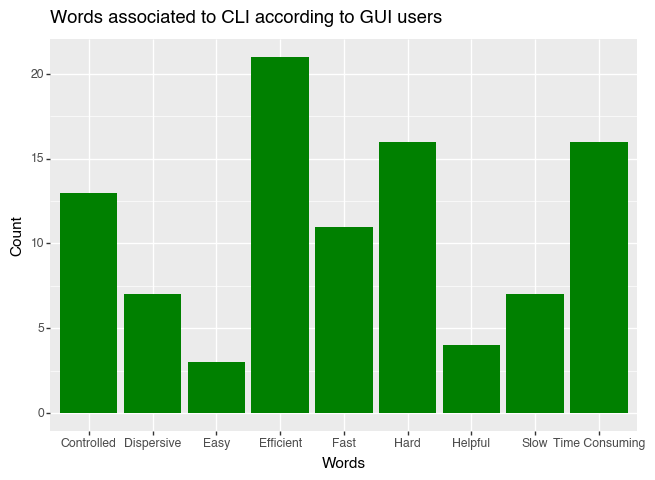
\includegraphics[width=0.75\linewidth]{WordsCLIFromGUI}\\
		\caption{CLI user words for GUI}
		\label{fig: 18}
	\end{figure}
\newpage
%Danny
\subsection{Experiment results}
The data displayed in the subsection will be regarding the experiment that was conducted among the IT students. We derived three plots in total which are most relevant to our research paper. Here we have shown the average time of completion in seconds between the two interfaces, the time it took for each participant in our experiment finishing the assignment through each interface.\\
		%EXPERIMENT
		
	To have a better overview and make the calculation of the average of all the students who completed our assignment, we converted the minutes we had recorded to seconds. That way it is easier to see the different times that people using the CLI and GUI had for the completion of the experiment. On x-axis we have the interface that was used for the completion and on the y-axis the average seconds it took the students. (figure.19)
\begin{figure}[H]
	\centering
	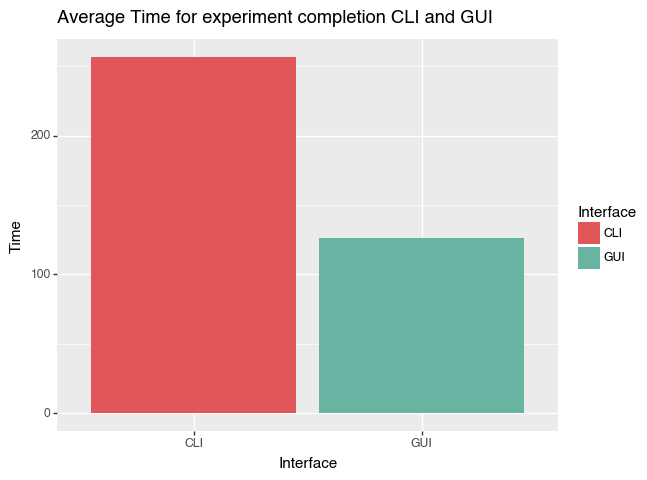
\includegraphics[width=0.75\linewidth]{ExperimentAverageTime}\\
	\caption{Average time for completing the experiment}
	\label{fig: 19}
\end{figure}
%END


%CHANGE%
In the following figure (figure.20) we have displayed all the completions of our assignment among all the candidates who used the CLI. Here we decided to keep the minutes and not convert to seconds since it has a better overview in this case of the actual times it took people.
%ON TOP%


%EXPERIMENT
\begin{figure}[H]
	\centering
	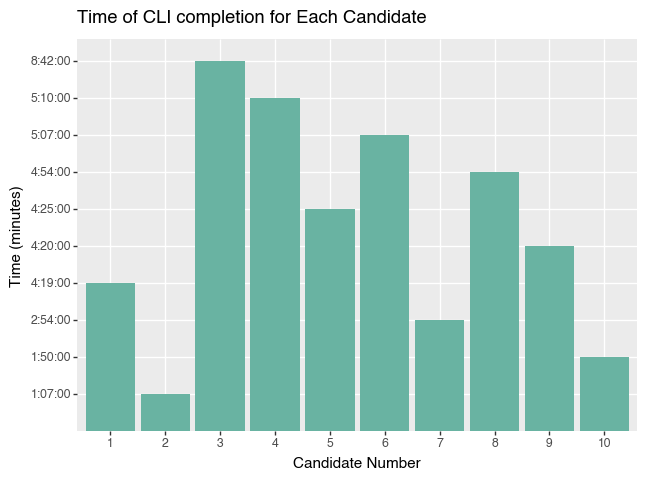
\includegraphics[width=0.75\linewidth]{ExperimentCli}\\
	\caption{Experiment completed through the command line interface}
	\label{fig: 20}
\end{figure}

Below, we have displayed the results of the people who finished the assignment with the GUI. As previously mentioned, all candidates who participated in our experiment had to complete the assignment with both interfaces.

%EXPERIMENt
\begin{figure}[H]
	\centering
	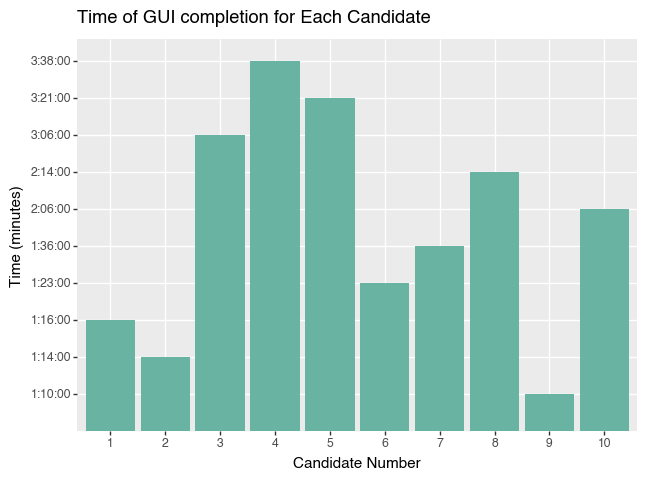
\includegraphics[width=0.75\linewidth]{ExperimentGui}\\
	\caption{Experiment completed through the graphical user interface}
	\label{fig: 21}
\end{figure}

	%Survery results%
	%Experiment results%
	%Data analysis%
	\newpage
	\section{Discussion}
	%Result interpration%
	%Evaluate research questions%
	%Limitations -> Y factors%
	%further research%
	\section{Appendix}
	\section{Acknowledgment}


\printbibliography[title=References]

\end{document}          
